% Section content template for individual Educative lessons
% This file contains the actual content for a specific section
% Generated from Educative API section content

% Section: Use Case Diagram for the Online Blackjack Game
% Section ID: 5466181593202688
% Section Slug: use-case-diagram-for-the-online-blackjack-game
% Generated: 2025-12-12T12:54:35.391758

Let's build the use case diagram of theonline Blackjack game and understand the relationships between its main actors and system functions. First , we'll define the different elements of our system, followed by the main actors and their associated use cases.

\subsection{System}\label{cP3DA2FVfsFuTwFqqixwy}
\\
Our system is an online Blackjack game. It manages player interactions, game rounds, betting, and outcomes between players and dealers.

\subsection{Actors}\label{kxFtRFH2EYDl4tVZpjsls}
\\
Now, we'll define the main actors of our Blackjack game.

\subsubsection{Primary actor}\label{IPDUHtML9sqQwKmSe8JY2}

\begin{itemize}
\item
\protect\phantomsection\label{-VknleK5wdxWZumDCJo0T}
\textbf{Player:} The main participant in the game. A player can join games, place bets, perform in-game actions (hit, stand, resign), and manage their account (create, update, reset password, cancel membership, login/logout).
\end{itemize}

\subsubsection{Secondary actor}\label{GWhiEOEVSdDmBizndxOiY}

\begin{itemize}
\item
\protect\phantomsection\label{NRPbwJraOhjj7b9ec5UQs}
\textbf{Dealer:} The dealer manages the Blackjack table, controls the game flow, deals cards, enforces rules, and completes payouts. The dealer may also manage player accounts (e.g., block members).
\end{itemize}

\subsection{Use cases}\label{bhS0oT5A37lHzjUgQ7tbU}
\\
This section will define the use cases for the Blackjack game. We have listed the use cases according to their interactions with a particular actor.
\begin{quote}
\textbf{Note:} Some use cases will occur multiple times because they are shared among different actors in the system.
\end{quote}
\subsubsection{Player}\label{ns2oMYLLRRM_8ZiVCnlKs}

\begin{itemize}
\item
\protect\phantomsection\label{bOuaa0UfFh2UNxnM4MCTW}
\textbf{Create account:} To register a new player profile in the Blackjack system.
\item
\protect\phantomsection\label{NYTQnsp1mP_ZvNRAgryMi}
\textbf{Login/Logout:} To securely log in or out of the Blackjack game.
\item
\protect\phantomsection\label{342S2KOa70ATJ0K2X_PWE}
\textbf{Update Account:} To edit personal account details, such as username, password, and contact information, or even cancel membership.
\item
\protect\phantomsection\label{V-P9duRbX75CVAYXOY-SD}
\textbf{View Open Games:} Browse a list of available Blackjack games waiting for players to join.
\item
\protect\phantomsection\label{M6gxXSGiiwCOhqRhFsj83}
\textbf{Join a Game:} To enter an open Blackjack table as a participant.
\item
\protect\phantomsection\label{QnfoaWwoFYsMepdwPJTNs}
\textbf{Place Bet:} To wager a specified amount for the current round.
\item
\protect\phantomsection\label{g113dX1esz76EmzWZiSo9}
\textbf{Hit:} To request an additional card from the dealer during a round.
\item
\protect\phantomsection\label{82Jeyq4oaktanQOCCT8hf}
\textbf{Stand:} To end the turn and retain current cards, awaiting game outcome.
\item
\protect\phantomsection\label{EGc_S2dUs8Iub9r9pGiD-}
\textbf{Resign Game:} To leave an active game before it is finished.
\end{itemize}

\subsubsection{Dealer}\label{br6YRHPg_mmFSD79mNrfK}

\begin{itemize}
\item
\protect\phantomsection\label{RVkIDkn1EwV67-u4nz5_J}
\textbf{Create Account:} To register a new dealer profile in the system.
\item
\protect\phantomsection\label{YalGHLVCe3fZeICkdvvCZ}
\textbf{Login/Logout:} To access or exit the dealer interface with credentials.
\item
\protect\phantomsection\label{uMfUQzm2I9Suv8IVaiGg4}
\textbf{Manage Account:} To oversee player accounts, including blocking a member from a game, and cancel their memberships.
\item
\protect\phantomsection\label{yQ7tVzztFVxqtR94pWtOC}
\textbf{Create New Game:} To set up a new Blackjack table or game round.
\item
\protect\phantomsection\label{amLFykGBsBwH-Zikwa7Lj}
\textbf{View Open Games:} To monitor all open games and wait for players.
\item
\protect\phantomsection\label{8AMHwaJnGU770XjHtM7rM}
\textbf{Create Hands:} To deal two cards to each player and the dealer at the start of a round.
\item
\protect\phantomsection\label{SUkiPY4JLdh9Pixwq77TA}
\textbf{Draw Card:} To add a card to any hand during gameplay.
\item
\protect\phantomsection\label{lidw9-ARxKNM1oFtSiqLV}
\textbf{Collect or Payout:} To settle bets by collecting losses or awarding winnings at the end of each round.
\end{itemize}

\subsection{Relationships}\label{4z8iTfs9KtUocdUwZSKN5}
\\
This section describes the relationships between and among actors and their use cases.

\subsubsection{Associations}\label{FJ0LyQABQpWK3XnUvhppG}
\\
The table below shows the association relationship between actors and their use cases.

\begin{center}
{\def\LTcaptype{none} % do not increment counter
\begin{longtable}[]{@{}
>{\raggedright\arraybackslash} p{(\linewidth - 2\tabcolsep) * \real{0.5000}}
>{\raggedright\arraybackslash} p{(\linewidth - 2\tabcolsep) * \real{0.5000}}@{}}
\toprule\noalign{}
\endhead
\bottomrule\noalign{}
\endlastfoot
\begin{minipage}[t]{\linewidth}\raggedright
\textbf{Player}
\end{minipage} & \begin{minipage}[t]{\linewidth}\raggedright
\textbf{Dealer}
\end{minipage} \\
\begin{minipage}[t]{\linewidth}\raggedright
Create account
\end{minipage} & \begin{minipage}[t]{\linewidth}\raggedright
Create account
\end{minipage} \\
\begin{minipage}[t]{\linewidth}\raggedright
Login/Logout
\end{minipage} & \begin{minipage}[t]{\linewidth}\raggedright
Login/Logout
\end{minipage} \\
\begin{minipage}[t]{\linewidth}\raggedright
Update account
\end{minipage} & \begin{minipage}[t]{\linewidth}\raggedright
Manage account
\end{minipage} \\
\begin{minipage}[t]{\linewidth}\raggedright
View open games
\end{minipage} & \begin{minipage}[t]{\linewidth}\raggedright
Create a new game
\end{minipage} \\
\begin{minipage}[t]{\linewidth}\raggedright
Join game
\end{minipage} & \begin{minipage}[t]{\linewidth}\raggedright
View open games
\end{minipage} \\
\begin{minipage}[t]{\linewidth}\raggedright
Place bet
\end{minipage} & \begin{minipage}[t]{\linewidth}\raggedright
Create hands
\end{minipage} \\
\begin{minipage}[t]{\linewidth}\raggedright
Hit
\end{minipage} & \begin{minipage}[t]{\linewidth}\raggedright
Draw card
\end{minipage} \\
\begin{minipage}[t]{\linewidth}\raggedright
Stand
\end{minipage} & \begin{minipage}[t]{\linewidth}\raggedright
Collect or payout
\end{minipage} \\
\begin{minipage}[t]{\linewidth}\raggedright
Resigns a game
\end{minipage} & \begin{minipage}[t]{\linewidth}\raggedright
-
\end{minipage} \\
\end{longtable}
}
\end{center}

\subsubsection{Include}\label{qxqhLC0efO3tk7A4JhCvF}
\\
Include relationships that capture mandatory, reusable behavior. They help avoid repetition: shared logic is modeled as a separate use case and included wherever needed.
\\
\textbf{Examples in the online Blackjack game:}

\begin{itemize}
\item
``Draw a card'' is included in both:

\begin{itemize}
\item
\textbf{Create hands:} When a new round starts, cards must be drawn for each participant (players and dealer).
\item
\textbf{Hit:} The system draws a card when a player requests an extra card.
\end{itemize}
\item
``Stand'' includes ``Collect or payout''\textbf{:}

\begin{itemize}
\item
After a player stands, the game outcome is evaluated, and payouts or collections are always processed as the next step.
\end{itemize}
\end{itemize}

\subsubsection{Extend}\label{VEs5zgo0aKNyTtpv0yfI1}
\\
Extend relationships represent optional or conditional behavior that occurs only under certain conditions or as a specific extension of the base use case.
\\
\textbf{Examples in the online Blackjack game:}

\begin{itemize}
\item
``Manage an account'' (for the dealer) is a general use case for managing player accounts.

\begin{itemize}
\item
``Block member'' and ``Cancel membership''are specific actions that extend ``Manage an account,'' as they are specialized cases triggered only when required.
\end{itemize}
\item
``Update an account'' (for the player) is the general use case for personal account changes.

\begin{itemize}
\item
``Cancel membership'' extends ``Update an account,'' as canceling one's membership or resetting one's password are conditional flows, not always part of every account update.
\end{itemize}
\end{itemize}

\subsection{Use case diagram}\label{QJOLSWrtsvNju5uS8JBOU}
\\
Here's the use case diagram of the Blackjack game:

\begin{figure}[htbp]
 \centering
 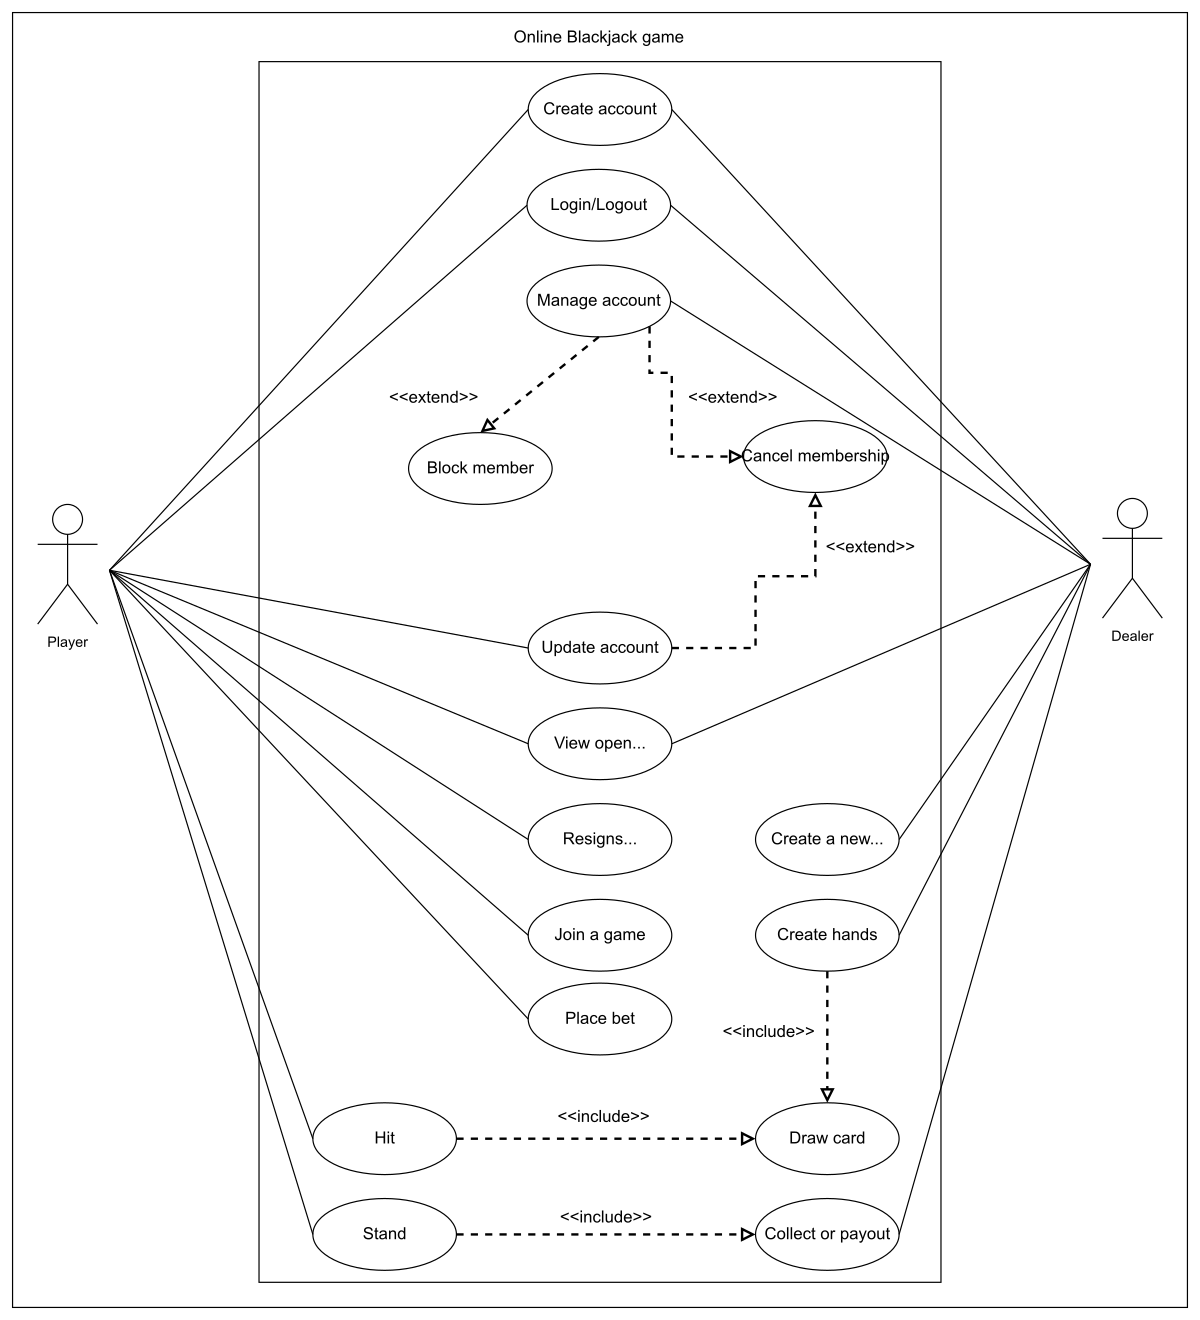
\includegraphics[width=0.5\textwidth]{Images/chapter_12/section_5466181593202688/6302763901124608.png}
 \caption{The use case diagram for the Blackjack game}
\end{figure}

In the next lesson, we will discuss the class diagram with a detailed explanation of all classes and their relationship with each other.

% End of section content